% !TeX root = ../TFG_LaTeX.tex
\section{Transformacions de Möbius}

\begin{adjustwidth}{1cm}{1cm}

    Les transformacions de Möbius constitueixen una de les famílies més bàsiques i, alhora, més importants de funcions en anàlisi complexa. Es tracta d'aplicacions definides mitjançant expressions racionals molt senzilles, però que presenten una estructura geomètrica especialment rica. Aquestes funcions apareixen de manera natural en molts problemes de la teoria de funcions complexes.

    Un dels principals interessos d'aquestes transformacions és que permeten estudiar com es comporten determinades regions del pla complex sota aplicacions conformes. En particular, són una eina fonamental per a transformar dominis complicats en altres més manejables, com el disc unitat o el semiplà superior. D'aquesta manera, les transformacions de Möbius serveixen com a canvis de coordenades que simplifiquen l'estudi de problemes analítics i geomètrics.

    A més, aquestes aplicacions estan estretament relacionades amb la geometria de l'esfera de Riemann, amb els automorfismes del disc unitat i amb la geometria hiperbòlica. A més, la seua classificació segons el comportament dels seus punts fixos és també molt útil per a analitzar la dinàmica holomorfa. Per aquest motiu, el seu estudi no sols és important dins de l'anàlisi complexa clàssica, sinó que també apareix en altres àrees com la geometria, la teoria de sistemes dinàmics, la teoria d'operadors i algunes aplicacions físiques on intervenen canvis conformes o simetries.

    En aquesta secció introduirem les transformacions de Möbius i estudiarem les seues propietats principals.

    Per a una exposició més detallada de les transformacions de Möbius i les seues propietats geomètriques, es poden consultar \cite[Cap. 3, Secció 3]{ahlfors}, \cite[Cap. III, Secció 3]{conway}, \cite[Cap. II, Secció 7]{gamelin}, i \cite{needham}.

    \begin{subsection}{Definició i propietats}

    \begin{definicio}
        Una \textbf{transformació de Möbius} és una funció de la forma 
        \begin{equation}
        f(z) = \frac{az + b}{cz + d}
        \label{eq:mobius}
        \end{equation} on $a,b,c,d$ són constants complexes que satisfan la condició $ad-bc \neq 0$. 

        El domini en $\mathbb{C}$ d'aquestes funcions ve donat per $\mathbb{C}\backslash\{\frac{-d}{c}\}$, però també podem estendre-les a $\mathbb{C}^*$ i considerar funcions $f:\mathbb{C}^*\to \mathbb{C}^*$ si definim 
        \[
            f(\infty)=
            \begin{cases}
                a/c & \text{ si } c\neq 0 \\
                \infty & \text{ si } c=0
            \end{cases}, \qquad \text{ i si } c\neq 0, \; \; f(-d/c)=\infty.
        \]
        
        
        La condició $ad-bc\neq 0$ simplement garanteix que $$f'(z) = \frac{ad - bc}{(cz + d)^2} \neq 0,$$ i per tant, que $f(z)$ no és constant. A més, si multipliquem totes les constants $a, b, c, d$ pel mateix paràmetre complex $\lambda$, arribem a la mateixa transformació de Möbius. Per tant, diferents eleccions de constants $a, b, c, d$ poden portar a la mateixa transformació.  
    \end{definicio}

        Un tipus especial de transformacions de Möbius són les \textbf{transformacions afins}, de la forma $f(z)=az+b$, on $a \neq 0$, i dins d'aquestes trobem les \textbf{translacions}, de la forma $f(z)=z+b$, i les \textbf{dilatacions}, de la forma $f(z)=az$.

        Altre tipus important de transformació és la \textbf{inversió}, que segueix la forma $f(z)=1/z$.

        \bigskip

    \begin{exemples}
        \leavevmode
        \begin{itemize}
            \item La identitat $f(z)=z$ és una transformació afí que a la vegada també és translació i dilatació, tot i ser un cas degenerat, perquè és una translació $z\mapsto z+b$ amb $b=0$ i és una dilatació $z\mapsto az$ amb $a=1$. 
            \item L'aplicació $f(z)=3z+2$ és una transformació afí, però no és ni translació ni dilatació.
        \end{itemize}  
    \end{exemples}


    Per tant, les translacions i les dilatacions envien l'infinit en ell mateix, i les inversions intercanvien el zero i l'infinit. D'eixa forma, les transformacions de Möbius es poden veure com una transformació del propi pla a un altre estat del mateix pla.

    \begin{figure}[H]
        \centering
        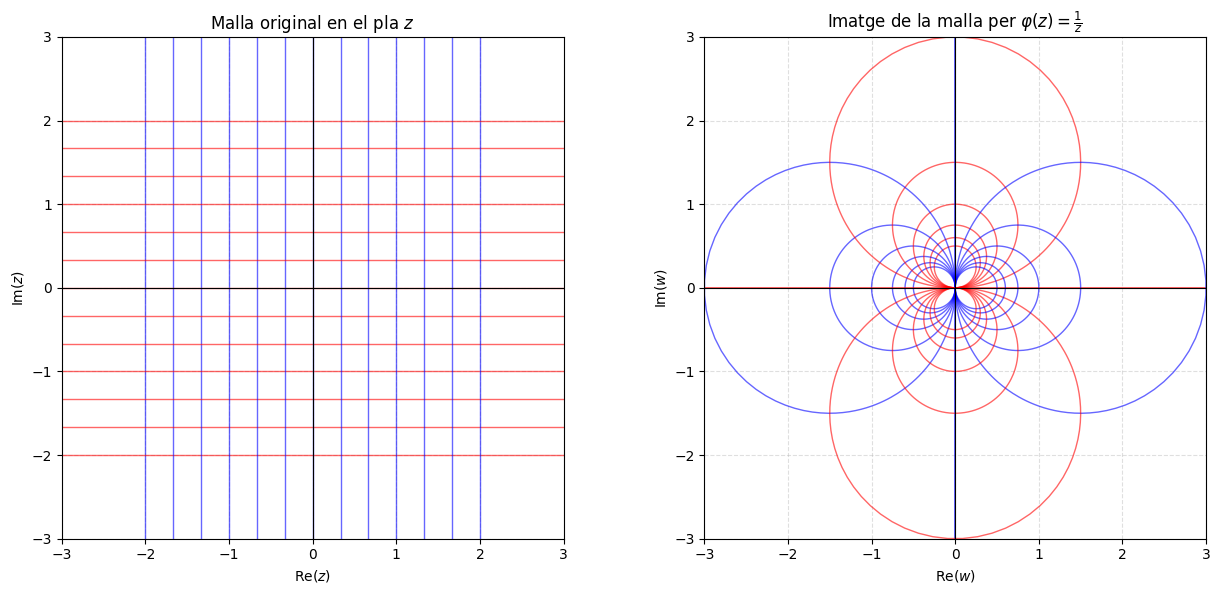
\includegraphics[width=0.65\textwidth]{pictures/funcio1entrez.png}
        \begin{adjustwidth}{1cm}{1cm}
        \caption{Imatge de $f(z)=1/z$ aplicada a rectes horitzontals i verticals.}
        \label{fig:mobius1} 
        \end{adjustwidth}
    \end{figure}
        

    \begin{nota}
        Per altra banda, també es pot considerar una transformació de Möbius com una funció $f(z)=\frac{az+b}{cz+d}$ amb domini $\mathbb{C}$ si $c=0$ o domini $\mathbb{C}\backslash\{\frac{-d}{c}\}$ si $c\neq0$, també complint la condició $ad-bc\neq 0$.

        Així, amb aquesta forma de definir $f$, tenim que és conforme en el seu domini, o com ja hem vist en el corol·lari \ref{nota_conf_sii_holomorfa}, és holomorfa en el seu domini.
    \end{nota}
    

    Altra propietat interessant de les transformacions de Möbius és la que s'exposa a continuació.

    \begin{proposicio}
            La inversa d'una transformació de Möbius torna a ser una transformació de Möbius.
    \end{proposicio}

    \begin{proof}
        Si 
            \[
            w=\frac{az+b}{cz+d}
            \]
            on $ad-bc \neq 0$, aleshores 
            \[
                w(cz+d)=az+b \iff z(cw-a)= -dw+b \iff z=\frac{-dw+b}{cw-a},
            \]
            i la condició $(-d)(-a)-bc \neq 0$ és la mateixa que $ad-bc \neq 0$.

            Aquest fet demostra, efectivament, que les transformacions de Möbius són aplicacions bijectives del pla complex ampliat en ell mateix.
    \end{proof}

    És igualment important que la composició de dues transformacions de Möbius també torna a ser una transformació de Möbius.

    \begin{proposicio}
        Si $f(z)=\frac{az+b}{cz+d}$ i $g(z)=\frac{\alpha z+\beta}{\gamma z+\delta}$ són dues transformacions de Möbius, amb $ad-bc \neq 0$ i $\alpha\delta-\beta\gamma \neq 0$, aleshores es té que $f\circ g$ també és una transformació de Möbius i $f(g(z))=\frac{\hat{a}z+\hat{b}}{\hat{c}z+\hat{d}}$ amb $\hat{a}\hat{d}-\hat{b}\hat{c} \neq 0$.
        \label{comp_de_mob_es_mob}
    \end{proposicio}

    \begin{proof}
        Tenim que 
        \[
            f(g(z))=\frac{a((\alpha z+\beta)/(\gamma z+\delta))+b}{c((\alpha z+\beta)/(\gamma z+\delta))+d}=\frac{(a\alpha+b\gamma)z+a\beta+b\delta}{(c\alpha+d\gamma)z+c\beta+d\delta}=\frac{\hat{a}z+\hat{b}}{\hat{c}z+\hat{d}},
        \]
        on $\hat{a}=(a\alpha+b\gamma), \hat{b}=(a\beta+b\delta), \hat{c}=(c\alpha+d\gamma), \hat{d}=(c\beta+d\delta)$.

        A més, la condició $\hat{a}\hat{d}-\hat{b}\hat{c}$, la qual, si la desenvolupem, queda com
        \[
            (a\alpha+b\gamma)(c\beta+d\delta)-(a\beta+b\delta)(c\alpha+d\gamma) \neq 0
        \]
        ve donada per les dues anteriors, ja que si factoritzem l'expressió anterior arribem a 
        \[
            (a\alpha+b\gamma)(c\beta+d\delta)-(a\beta+b\delta)(c\alpha+d\gamma)=
         \]
         \[
            =\cancel{a\alpha c\beta}+a\alpha d\delta +b\gamma c\beta +\cancel{b\gamma d\delta}-\cancel{a\beta c\alpha}-a\beta d\gamma-b\delta c\gamma-\cancel{b\delta d\gamma}=
         \]
         \[   
            =(ad-bc)(\alpha\delta-\beta\gamma) \neq 0.
        \]
        Per tant, tenim efectivament que $f(g(z))$ és una transformació de Möbius.
    \end{proof}

    \begin{nota}
         Gràcies a la proposició \ref{comp_de_mob_es_mob}, es pot afirmar que les transformacions de Möbius amb la composició té estructura de grup, que denotarem com $(TM,\circ)$.
    \end{nota}
   
    Notem que les transformacions de Möbius es poden identificar amb matrius $2\times2$ amb determinant no nul i, conseqüentment, la composició de transformacions de Möbius es correspon amb la multiplicació de matrius $2\times 2$. En efecte, 

    \[
        \begin{pmatrix}
            a & b \\
            c & d
        \end{pmatrix}
        \begin{pmatrix}
            \alpha & \beta \\
            \gamma & \delta
        \end{pmatrix} = 
        \begin{pmatrix}
            a\alpha+b\gamma & a\beta+b\delta \\
            c\alpha+d\gamma & c\beta+d\delta
        \end{pmatrix}.
    \]
    La primera i la segona matriu són les associades a les transformacions $f$ i $g$, respectivament, i la tercera és la matriu associada a la transformació $f \circ g$.

    Es veu clarament que la condició $ad-bc \neq 0$ és simplement demanar que la matriu associada a la transformació siga invertible.

    Aquest fet pot ser reformulat en termes de la teoria de grups. Fent la assignació matriu-transformació esmentada abans, obtenim l'homomorfisme entre grups
    \[
        \varphi : GL(2,\mathbb{C}) \to (TM,\circ),
    \]
    on $GL(2,\mathbb{C})$ és el grup de matrius $2\times 2$ invertibles amb coeficients complexos, amb operació el producte de matrius.

    Efectivament, $\varphi$ és un homomorfisme de grups, perquè per a tot $A,B$ en $GL(2,\mathbb{C})$ es verifica que
    \[
        \varphi(A)\circ \varphi(B) = \varphi(AB),
    \]
    com ja hem dit abans.

    Ara bé, l'homomorfisme no és injectiu, ja que $\varphi(A)=\varphi(\lambda A)$, per a tot $\lambda$ complex no nul.

    No obstant això, prenent el subgrup projectiu de $GL(2,\mathbb{C})$, que és 
    \[
        PGL(2,\mathbb{C})=GL(2,\mathbb{C})/Ker\{\varphi\}=GL(2,\mathbb{C})/\{\lambda I: \lambda\neq 0\},
    \]
    ja tenim que l'homomorfisme entre grups
    \[
        \hat{\varphi} : PGL(2,\mathbb{C}) \to (TM,\circ)
    \]
    és injectiu i també sobrejectiu. Per tant, $\hat{\varphi}$ és un isomorfisme de grups.


    \end{subsection}

    \begin{subsection}{Propietats geomètriques}

    En el següent teorema veurem que una transformació de Möbius queda completament determinada de forma única si triem 3 punts de $\mathbb{C}^*$ i elegim quines volem que siguen les seues imatges, també en $\mathbb{C}^*$.

    \begin{teorema}
        Donats tres punts $z_0, z_1, z_2$ en el pla complex ampliat, i donats tres valors $w_0, w_1, w_2$ també en el pla complex ampliat, hi ha una única transformació de Möbius $w=w(z)$ tal que $w_0=w(z_0), w_1=w(z_1), \text{i } w_2=w(z_2)$.
    \end{teorema}

    \begin{proof}
        Per tal d'establir l'existència, n'hi ha prou amb demostrar que es poden enviar qualsevol tres punts distints al $0$, al $1$ i al $\infty$, respectivament.

        En efecte, si $f$ envia $z_0, z_1, z_2$ a $0,1,\infty$, i $g$ envia $w_0, w_1, w_2$ també a $0,1,\infty$, aleshores la composició $g^{-1} \circ f$, que com s'ha provat abans és també una transformació de Möbius, envia $z_0, z_1, z_2$ a $w_0, w_1, w_2$, i per tant $g^{-1}\circ f$ és la transformació buscada.
        
        Ara bé, si cap dels tres punts $z_0, z_1, z_2$ és l'$\infty$, una transformació que realitza això està donada explícitament per

        \begin{equation}
            w = f(z) = \frac{z - z_0}{z - z_2} \cdot \frac{z_1 - z_2}{z_1 - z_0}.
            \label{eq1punts3}
        \end{equation}

        Si algun dels $z_j$ és l'$\infty$, definim $f(z)$ fent tendir $z_j$ a l'$\infty$ en la fórmula anterior. Per exemple, si $z_0 = \infty$, es pot escriure el segon membre de (\ref{eq1punts3}) com

        \[
            \frac{(z/z_0) - 1}{z - z_2} \cdot \frac{z_1 - z_2}{(z_1/z_0) - 1}
        \]

        i prenent el límit quan $z_0 \to \infty$, s'obté

        \[
            w = f(z) = \frac{z_1 - z_2}{z - z_2}.
        \]

        Aquesta transformació envia $\infty, z_1, z_2$ a $0,1,\infty$, respectivament. Existeixen fórmules similars per als casos en què $z_1 = \infty$ o $z_2 = \infty$.

        Per a la unicitat, es suposa primer que $f(z)$ és una transformació de Möbius que fixa els punts $0,1,\infty$. Com que $f(\infty)=\infty$, la transformació resulta ser afí, és a dir, que és de la forma $f(z)=az+b$. De $f(0)=0$ s'obté $b=0$, i de $f(1)=1$ s'obté $a=1$. Així, $f(z)=z$ és la identitat.

        Ara es suposa que $g(z)$ i $h(z)$ són transformacions de Möbius que envien els punts $z_j$ als respectius $w_j$. Siga $k(z)$ la transformació que envia els $z_j$ a $0,1,\infty$. Aleshores $f := k \circ h^{-1} \circ g \circ k^{-1}$ fixa els punts $0,1,\infty$. Per tant $f$ és la identitat, i es pot dir que $g = h \circ k^{-1} \circ f \circ k = h \circ k^{-1} \circ k = h$. Això estableix la unicitat del teorema.
    \end{proof}

    \begin{exemple}
        Volem trobar la transformació de Möbius que envia els punts $z_0=0, z_1=1, z_2=i$ als punts $w_0=-i,w_1=-1,w_2=0$, respectivament.

        Aleshores, basant-se en el procediment de la prova del teorema anterior, considerem la transformació de Möbius $f(z)=\frac{(1-i)z}{(z-i)}$, que envia $z_0,z_1,z_2$ a $0,1,\infty$, respectivament.

        Anàlogament, considerem la transformació de Möbius $g(z)=\frac{(z+i)(-1)}{z(i-1)}=\frac{z+i}{(1-i)z}$, que envia $w_0,w_1,w_2$ a $0,1,\infty$, respectivament. La seua inversa també és transformació de Möbius i 
        \[
            w=g(z)=\frac{z+i}{(1-i)z} \iff z(1-i)w=z+i \iff z=g^{-1}(w)=\frac{i}{(1-i)w-1}.
        \]
        

        Així, la transformació de Möbius $\varphi(z):=g^{-1}\circ f$ envia $z_0,z_1,z_2$ a $w_0,w_1,w_2$, respectivament, i aquesta ve donada per 
        \[
            \varphi(z)=g^{-1}(f(z))=g^{-1}\left(\frac{(1-i)z}{(z-i)}\right)=\left(\frac{i}{(1-i)\left(\frac{(1-i)z}{(z-i)}\right)-1}\right)=
        \]
        \[
            =\left(\frac{i(z-i)}{(1-i)^2(z)-(z-i)}\right)=\left(\frac{iz+1}{(-2i-1)z+i}\right)=\left(\frac{z-i}{(i-2)z+1}\right).
        \]
        En efecte, $\varphi(0)=-i$, $\varphi(1)=-1$, i $\varphi(i)=0$. Gràficament, 

        \begin{figure}[H]
        \centering
        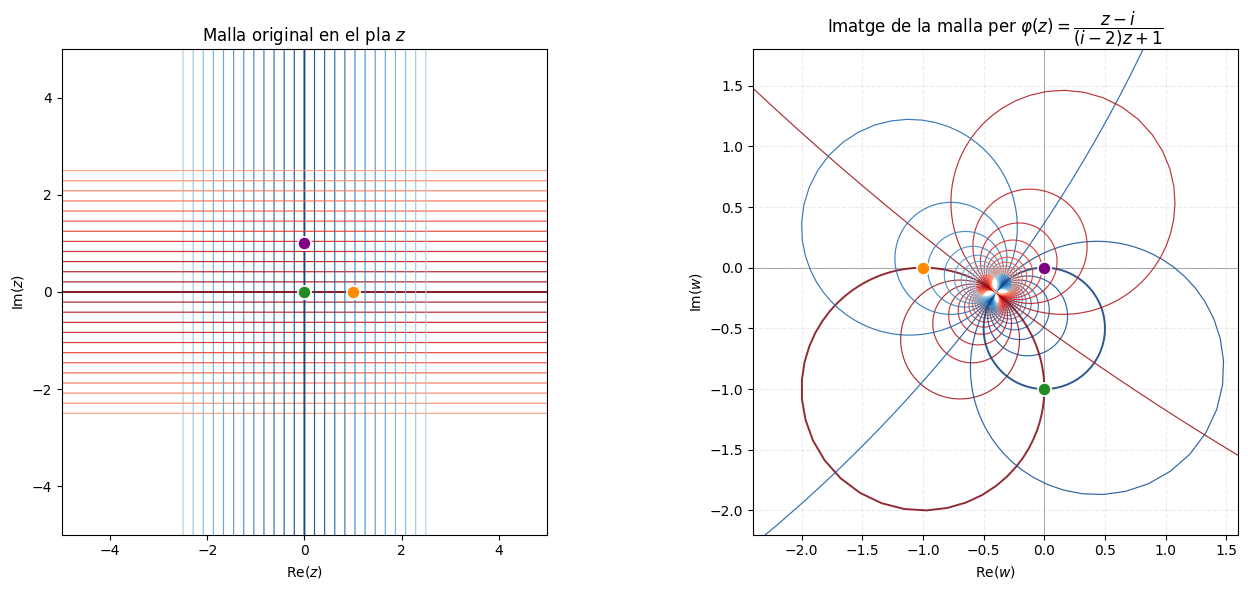
\includegraphics[width=0.9\textwidth]{pictures/exemple_funcio_envia_3_punts_en_3_punts.png}
        \begin{adjustwidth}{1cm}{1cm}
        \caption{Imatge de $\varphi(z)=\frac{z-i}{(i-2)z+1}$ aplicada a rectes horitzontals i verticals.}
        \label{fig:exemple_funcio_envia_3_punts_en_3_punts} 
        \end{adjustwidth}
    \end{figure}

    En les imatges anteriors, també veiem dibuixats els punts $z_0=0$ i $w_0=\varphi(z_0)=-i$ en verd, els punts $z_1=1$ i $w_1=\varphi(z_1)=-1$ en taronja, i els punts $z_2=i$ i $w_2=\varphi(z_2)=0$ en morat.
    \end{exemple}

    \begin{teorema}
        Tota transformació de Möbius és una composició de dilatacions, translacions i inversions.
    \end{teorema}

    \begin{proof}
        Siga $f$ la nostra transformació de Möbius. Primer considerem el cas que la transformació fixa l'$\infty$. En eixe cas, com ja hem vist, $f$ té la forma $f(z)=az+b$, on $a\neq 0$, i per tant això és la composició de la dilatació $z \mapsto az$ i la translació $z \mapsto z+b$:
        \[
            z \mapsto az \mapsto az+b.
        \] 

        En canvi, si $f(\infty)\in \mathbb{C}$, aleshores $f(z)=\frac{az+b}{cz+d}$, on $c\neq 0$. En aquest cas podríem dividir tots els paràmetres entre $c$, i per tant podem assumir $c=1$. D'aquesta forma, escrivim $f$ com una composició d'una translació, una inversió, una dilatació i una translació de la forma
        \[
            z \mapsto z+d \mapsto \frac{1}{z+d} \mapsto \frac{b-ad}{z+d} \mapsto a+\frac{b-ad}{z+d}=\frac{az+b}{z+d}.
        \]

        Això acaba de probar el teorema.
    \end{proof}

    A continuació es provarà un teorema que és essencial en la teoria de transformacions de Möbius, però primer és important recordar que qualsevol recta en $\mathbb{C}$ pot ser vista com una circumferència en $\mathbb{C}^*$ si se li afegeix el punt $\infty$. Una forma de visualitzar aquest fet és que si tenim un punt $z_0$ que pertany a una recta, eixa recta pot ser vista com el límit quan el radi tendeix a infinit de les circumferències situades totes al mateix costat de la recta i tangents a la pròpia recta en el punt $z_0$. Visualment,

    \begin{figure}[H]
        \centering
        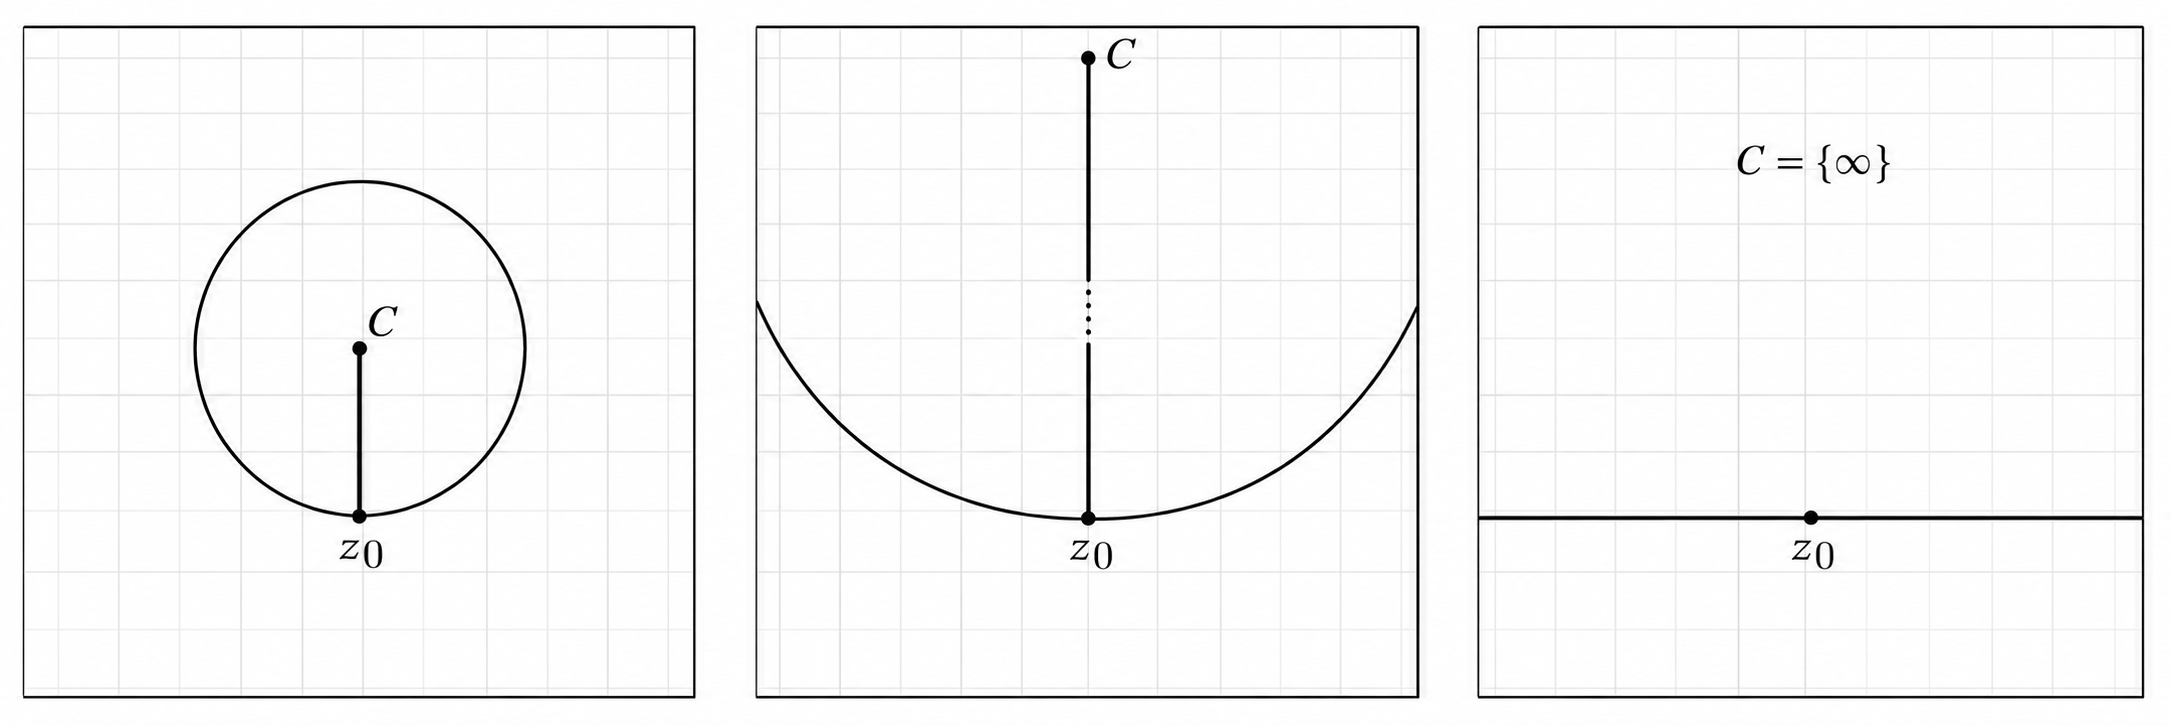
\includegraphics[width=0.9\textwidth]{pictures/recta_es_circ_infinita.png}
        \begin{adjustwidth}{1cm}{1cm}
        \caption{Representació de que una recta és una circumferència en $\mathbb{C}^*$.}
        \label{fig:recta_es_circ_infinita} 
        \end{adjustwidth}
    \end{figure}

    \begin{teorema}
        Una transformació de Möbius transforma circumferències de $\mathbb{C}^*$ en circumferències de $\mathbb{C}^*$.
        \label{tm_circ_en_circ}
    \end{teorema}

    \begin{proof}
        És suficient provar-ho per a translacions, per a dilatacions i per a inversions, ja que com s'ha provat en el teorema anterior, qualsevol transformació de Möbius és composició d'estes.

        Primerament, que les translacions i les dilatacions transformen circumferències en circumferències està clar, perquè el punt infinit es fixa i tots els altres punts funcionen igual que qualsevol translació o dilatació en $\mathbb{C}$. Per tant, es suficient veure que la inversió $f(z)=\frac{1}{z}$ transforma circumferències en circumferències. 

        Ara bé, anem a diferenciar dos casos, depenent de si la circumferència passa per l'$\infty$ o no. En el primer cas, la circumferència té una equació de la forma $|z-a|^2=r^2$, on $a\in \mathbb{C}$ és el centre de la circumferència i $r>0$ és el seu radi. Així, la imatge d'aquesta circumferència per $f$ és el conjunt $|1-af(z)|^2=r^2|f(z)|^2$, i suposant que $z\neq 0$, 
        \[
            \begin{aligned}
                0 &= |1-af(z)|^2-r^2|f(z)|^2 = (1-af(z))(\overline{1-af(z)})-r^2|f(z)|^2 = \\
                &= (|a|^2-r^2)|f(z)|^2-af(z)-\overline{af(z)}+1.
            \end{aligned}
        \]
        Anomenem $f(z)=u+iv$ on $u$ i $v$ són reals. Aleshores l'equació pren la forma  
        \begin{equation}
            (|a|^2-r^2)(u^2+v^2)+Au+Bv+1 = 0,
            \label{eq_circ_en_circ}
        \end{equation}
        on 
        \[
            A=-2\operatorname{Re}(a), \qquad B=2\operatorname{Im}(a)
        \]
        són constants reals. Si $r=|a|$, l'equació anterior representa una recta en el pla $\mathbb{C}$, i a més, com el punt $0$ formava part del domini de l'equació $|z-a|^2=r^2$, el punt $\infty=f(0)$ també es part de la imatge de la circumferència. Però pel comentari d'abans, una recta en $\mathbb{C}$ unit al punt $\infty$ és exactament una circumferència en $\mathbb{C}^*$.

        En el cas que $r\neq |a|$, no cal preocupar-se pel punt $z=0$, i l'equació (\ref{eq_circ_en_circ}) és una equació quadràtica en $u$ i en $v$ que, si anomenem $C:=|a|^2-r^2$ i $R:=\left(\frac{A}{2C}\right)^2+\left(\frac{B}{2C}\right)^2-\frac{1}{C}$, podem reformular com 
        \[
            \left(u+\frac{A}{2C}\right)^2+\left(v+\frac{B}{2C}\right)^2=R^2,
        \]
        i això es ben sabut que és l'equació d'una circumferència usual en $\mathbb{C}$ centrada en $-\frac{A}{2C} -i\frac{B}{2C}$ de radi $R$.

        Com a segon cas considerem que la nostra circumferència sí que passa per l'$\infty$, és a dir, que és una recta unida al punt $\infty$. Així, $f(\infty)=0$ i l'equació d'aquesta recta té la forma $Cx+Dy = E$, on $z=x+iy$ i $C,D,E$ són paràmetres reals. 

        Aleshores, com 
        \[
            f(x+iy)=\frac{1}{x+iy}=\frac{x}{x^2+y^2}+i \frac{-y}{x^2+y^2},
        \]
        la imatge de l'equació de la recta per $f$ és $\frac{Cx-Dy}{x^2+y^2}=E$, cosa que podem reescriure, si $(x,y)\neq 0$, com $E(x^2+y^2)=Cx-Dy$. Ara bé,  si $E\neq 0$, aleshores la recta inicial no passa pel $0$ i el que hem fet té sentit per a tots els punts de la recta, i eixa equació que hem posat és l'expressió de la circumferència 
        \[
            \left(x-\frac{C}{2E}\right)^2+\left(y+\frac{D}{2E}\right)^2=\left(\frac{\sqrt{C^2+D^2}}{2E}\right)^2,
        \]
        és a dir, la circumferència centrada en $\left(\frac{C}{2E},\frac{-D}{2E}\right)$ de radi $\frac{\sqrt{C^2+D^2}}{2E}$, i si $E=0$, aleshores la nostra recta inicial passa per $(x,y)=0$, i tenim que per una banda $f(0)=\infty$, i que per l'altra $f$ transforma la recta inicial (llevant el $0$) en la recta $y=\frac{C}{D}x$, que sumada a l'$\infty$ que obtenim com a imatge del $0$ ens fan una circumferència en $\mathbb{C}^*$.
    \end{proof}

    \end{subsection}

\end{adjustwidth}